\lab{QR 2: Least Squares and Computing Eigenvalues}{Least Squares and Computing Eigenvalues}
\label{lab:qr-applications}
\objective{Because of its numerical stability and convenient structure, the QR decomposition is the basis of many important and practical algorithms.
In this lab, we introduce linear least squares problems, tools in Python for computing least squares solutions, and two fundamental eigenvalue algorithms.
\\ \indent As in the previous lab, we restrict ourselves to real matrices and therefore use the transpose in place of the Hermitian conjugate.}

\section*{Least Squares} % ====================================================

A linear system $A\x = \b$ is \emph{overdetermined} if it has more equations than unknowns.
In this situation, there is no true solution, and $\x$ can only be approximated.

The \emph{least squares solution} of $A\x = \b$, denoted as $\widehat{\x}$, is the ``closest'' vector to a solution, meaning it minimizes the quantity $\|A\widehat{\x} - \b\|_2$.
% \footnote{The choice of the 2-norm is significant.}
In other words, $\widehat{\x}$ is the vector such that $A\widehat{\x}$ is projection of $\b$ onto the range of $A$, and can be calculated by solving the \emph{normal equation}:%
\footnote{See Volume I Chapter 3 for a formal derivation of the normal equation.}
\[A\trp A\widehat{\x} = A\trp \b\]

If $A$ is full rank, which it usually is in applications, its QR decomposition provides an efficient way to solve the normal equation.
Let $A = \widehat{Q}\widehat{R}$ be the reduced QR decomposition of $A$, so $\widehat{Q}$ is $m \times n$ with orthonormal columns and $\widehat{R}$ is $n \times n$, invertible, and upper triangular.
Since $\widehat{Q}\trp \widehat{Q} = I$, and since $\widehat{R}\trp$ is invertible, the normal equation can be reduced as follows (we omit the hats on $\widehat{Q}$ and $\widehat{R}$ for clarity):
%
\begin{align}
\nonumber
A\trp A\widehat{\x} &= A\trp \b \\ \nonumber
(Q R)\trp Q R  \widehat{\x}
&= (Q R)\trp \b \\ \nonumber
 R\trp Q\trp Q R  \widehat{\x}
&=  R\trp Q\trp \b \\ \nonumber
 R\trp R \widehat{\x}
&=  R\trp Q\trp \b \\
 R \widehat{\x}
&= Q\trp \b \label{eq:normal-equation-via-qr}
\end{align}

Thus $\widehat{\x}$ is the least squares solution to $A\x=\b$ if and only if $\widehat{R}\widehat{\x} = \widehat{Q}\trp\b.$
Since $\widehat{R}$ is upper triangular, this equation can be solved quickly with back substitution.

\begin{problem} % Solve the normal equations with QR.
Write a function that accepts an $m \times n$ matrix $A$ of rank $n$ and a vector $\b$ of length $n$.
Use the QR decomposition and Equation \ref{eq:normal-equation-via-qr} to solve the normal equation corresponding to $A\x = \b$.

You may use either SciPy's QR routine or one of your own routines from the previous lab.
In addition, you may use \li{la.solve_triangular()}, SciPy's optimized routine for solving triangular systems.

\label{prob:lstsq-via-qr}
\end{problem}

\subsection*{Fitting a Line} % ------------------------------------------------

The least squares solution can be used to find the best fit curve of a chosen type to a set of points.
Consider the problem of finding the line $y = ax + b$ that best fits a set of $m$ points $\{(x_k, y_k)\}_{k=1}^m$.
Ideally, we seek $a$ and $b$ such that $y_k = ax_k + b$ for all $k$.
The following linear system simultaneously represents all of these equations.
%
\begin{equation}
A\x =
\left[\begin{array}{cc}
x_1 & 1 \\
x_2 & 1 \\
x_3 & 1 \\
\vdots & \vdots \\
x_m & 1
\end{array}\right]
\left[\begin{array}{c} a \\ b \end{array}\right]
=
\left[\begin{array}{c} y_1 \\ y_2 \\ y_3 \\ \vdots \\ y_m \end{array}\right]
= \b
\label{eq:linear-least-squares}
\end{equation}
%
Note that $A$ has full column rank as long as not all of the $x_k$ values are the same.

Because this system has two unknowns, it is guaranteed to have a solution if it has two or fewer equations.
However, if there are more that two data points, the system is overdetermined if any set of three points are not collinear.
We therefore seek a least squares solution, which in this case means finding the slope $\widehat{a}$ and $y$-intercept $\widehat{b}$ such that the line $y = \widehat{a}x+\widehat{b}$ best fits the data.

Figure \ref{fig:line-fit-example} is a typical example of this idea where $\widehat{a} \approx \frac{1}{2}$ and $\widehat{b} \approx -3$.

\begin{figure}[H] % Linear regression example (without code).
    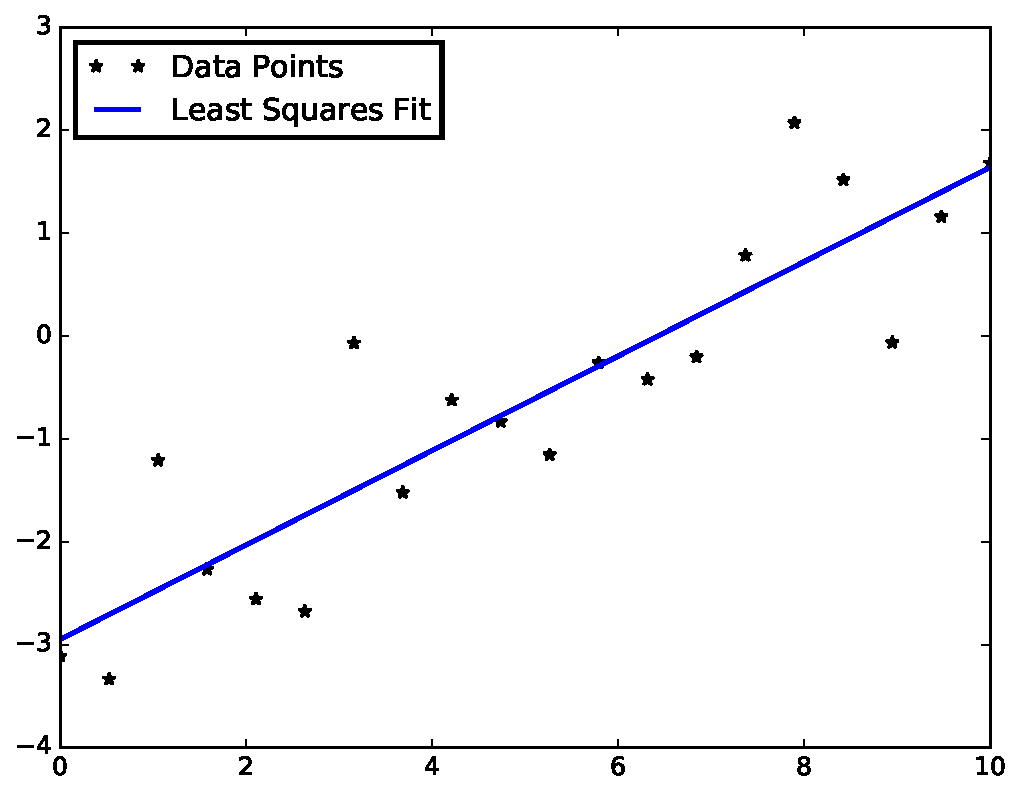
\includegraphics[width=.59\textwidth]{figures/line_fit_example.pdf}
    \caption{}
    \label{fig:line-fit-example}
\end{figure}

% TODO: Replacing this data set housing_prices.npy (average housing prices since 2000).
\begin{problem}
The file \texttt{housing.npy} contains the purchase-only housing price index, a measure of how housing prices are changing, for the United States from 2000 to 2010.%
\footnote{See \url{http://www.fhfa.gov/DataTools/Downloads/Pages/House-Price-Index.aspx}.}
Each row in the array is a separate measurement; the columns are the year and the price index, in that order.
To avoid large numerical computations, the year measurements start at 0 instead of 2000.

Find the least squares line that relates the year to the housing price index (i.e., let year be the $x$-axis and index the $y$-axis).

\begin{enumerate}
    \item Construct the matrix $A$ and the vector $\b$ described by Equation \ref{eq:linear-least-squares}.\\
    (Hint: the functions \li{np.vstack()}, \li{np.column_stack()}, and/or \li{np.ones()} may be helpful.)
    \item Use your function from Problem \ref{prob:lstsq-via-qr} to find the least squares solution.
    \item Plot the data points as a scatter plot.
    \item Plot the least squares line with the scatter plot.\\
\end{enumerate}
\end{problem}

\begin{info} % scipy.stats.linregress().
The least squares problem of fitting a line to a set of points is often called \emph{linear regression}, and the resulting line is called the \emph{linear regression line}.
SciPy's specialized tool for linear regression is \li{scipy.stats.linregress()}.
This function takes in an array of $x$-coordinates and a corresponding array of $y$-coordinates, and returns the slope and intercept of the regression line, along with a few other statistical measurements.

For example, the following code produces Figure \ref{fig:line-fit-example}.

\begin{lstlisting}
>>> import numpy as np
>>> from scipy.stats import linregress

# Generate some random data close to the line y = .5x - 3.
>>> x = np.linspace(0, 10, 20)
>>> y = .5*x - 3 + np.random.randn(20)

# Use linregress() to calculate m and b, as well as the correlation
# coefficient, p-value, and standard error. See the documentation for
# details on each of these extra return values.
>>> a, b, rvalue, pvalue, stderr = linregress(x, y)

>>> plt.plot(x, y, 'k*', label="Data Points")
>>> plt.plot(x, a*x + b, 'b-', lw=2, label="Least Squares Fit")
>>> plt.legend(loc="upper left")
>>> plt.show()
\end{lstlisting}
\end{info}

\subsection*{Fitting a Polynomial} % ------------------------------------------

Least squares can also be used to fit a set of data to the best fit polynomial of a specified degree.
Let $\{(x_k, y_k)\}_{k=1}^m$ be the set of $m$ data points in question.
The general form for a polynomial of degree $n$ is as follows:
\[
p_n(x) = c_n x^n + c_{n-1} x^{n-1} + \cdots + c_2 x^2 + c_1 x + c_0
\]
Note that the polynomial is uniquely determined by its $n+1$ coefficients $\{c_k\}_{k=0}^n$.
Ideally, then, we seek the set of coefficients $\{c_k\}_{k=0}^n$ such that
\[
y_k = c_n x_k^n + c_{n-1} x_k^{n-1} + \cdots + c_2 x_k^2 + c_1 x_k + c_0
\]
for all values of $k$.
These $m$ linear equations yield the following linear system:
\begin{equation}
A\x =
\left[\begin{array}{cccccc}
x_1^n & x_1^{n-1} & \cdots & x_1^2 & x_1 & 1 \\
x_2^n & x_2^{n-1} & \cdots & x_2^2 & x_2 & 1 \\
x_3^n & x_3^{n-1} & \cdots & x_3^2 & x_3 & 1 \\
\vdots & \vdots & & \vdots & \vdots & \vdots \\
x_m^n & x_m^{n-1} & \cdots & x_m^2 & x_m & 1 \\
\end{array}\right]
\left[\begin{array}{c}
c_n \\ c_{n-1} \\ \vdots \\ c_2 \\ c_1 \\ c_0
\end{array}\right]
=
\left[\begin{array}{c} y_1 \\ y_2 \\ y_3 \\ \vdots \\ y_m \end{array}\right]
= \b
\label{eq:polynomial-least-squares}
\end{equation}
%
If $m > n+1$ this system is overdetermined, requiring a least squares solution.

\subsubsection*{Working with Polynomials in NumPy} % - - - - - - - - - - - - -

The $m \times (n+1)$ matrix $A$ of Equation \ref{eq:polynomial-least-squares} is called a \emph{Vandermonde matrix}.%
\footnote{Vandermonde matrices have many special properties and are useful for many applications, including polynomial interpolation and discrete Fourier analysis.}
% a matrix with entries $a_{ij} = x_i^{n-j+1}$.
NumPy's \li{np.vander()} is a convenient tool for quickly constructing a Vandermonde matrix, given the values $\{x_k\}_{k=1}^m$ and the number of desired columns.

\begin{lstlisting}
>>> print(np.vander([2, 3, 5], 2))
[[2 1]
 [3 1]
 [5 1]]

>>> print(np.vander([2, 3, 5, 4], 3))
[[ 4  2  1]
 [ 9  3  1]
 [25  5  1]
 [16  4  1]]
\end{lstlisting}

NumPy also has powerful tools for working efficiently with polynomials.
The class \li{np.poly1d} represents a 1-dimensional polynomial.
Instances of this class are callable like a function.%
\footnote{Class instances can be made callable by implementing the \li{__call__()} magic method.}
The constructor accepts the polynomial's coefficients, from largest degree to smallest.

Table \ref{table:numpy-poly1d} lists the attributes and methods of the \li{np.poly1d} class.
See \url{http://docs.scipy.org/doc/numpy/reference/routines.polynomials.html} for a list of NumPy's polynomial routines.

\begin{table}[H]
\begin{tabular}{r|l}
    Attribute & Description \\
    \hline
    coeffs & The $n+1$ coefficients, from greatest degree to least. \\
    order & The polynomial degree ($n$). \\
    roots & The $n-1$ roots. \\
    \\
    Method & Returns \\
    \hline
    deriv() & The coefficients of the polynomial after being differentiated. \\
    integ() & The coefficients of the polynomial after being integrated (with $c_0 = 0$).
\end{tabular}
\caption{Attributes and methods of the \li{np.poly1d} class.}
\label{table:numpy-poly1d}
\end{table}
%
\begin{lstlisting}
# Create a callable object for the polynomial f(x) = (x-1)(x-2) = x^2 - 3x + 2.
>>> f = np.poly1d([1, -3, 2])
>>> print(f)
   2
1 x - 3 x + 2

# Evaluate f(x) for several values of x in a single function call.
>>> f([1, 2, 3, 4])
array([0, 0, 2, 6])

# Evaluate f(x) at 1, 2, 3, and 4 without creating f(x) explicitly.
>>> np.polyval([1, -3, 2], [1, 2, 3, 4])
array([0, 0, 2, 6])
\end{lstlisting}

\begin{problem} % Polynomial fitting.
The data in \texttt{housing.npy} is nonlinear, and might be better fit by a polynomial than a line.

Write a function that uses Equation \ref{eq:polynomial-least-squares} to calculate the polynomials of degree $3$, $6$, $9$, and $12$ that best fit the data.
Plot the original data points and each least squares polynomial together in individual subplots.
\\(Hint: define a separate, more refined domain with \li{np.linspace()} and use this domain to smoothly plot the polynomials.)

Instead of using Problem \ref{prob:lstsq-via-qr} to solve the normal equation, you may use \li{scipy.linalg.lstsq()}, demonstrated below.

\begin{lstlisting}
>>> from scipy import linalg as la

# Define A and b appropriately.

# Solve the normal equation using SciPy's least squares routine.
# The least squares solution is the first of four return values.
>>> x = la.lstsq(A, b)[0]
\end{lstlisting}

Compare your results to \li{np.polyfit()}.
This function receives an array of $x$ values, an array of $y$ values, and an integer for the polynomial degree, and returns the coefficients of the best fit polynomial of that degree.

\begin{comment}
\begin{lstlisting}
# Generate some random data close to the line y = x^2 - 3x + 2.
>>> x = np.linspace(0, 10, 20)
>>> y = x**2 - 3*x + 2 + np.random.randn(20)

# Use np.polyfit() to calculate the best fit 2nd degree polynomial.
>>> coeffs = np.polyfit(x, y, 2)

>>> domain = np.linspace(0, 10, 200)
>>> plt.plot(x, y, 'k*')
>>> plt.plot(domain, np.polyval(coeffs, domain))
>>> plt.show()
\end{lstlisting}
\end{comment}

\label{prob:polynomial-least-squares}
\end{problem}

\begin{warn} % Overfitting
Having more parameters in a least squares model is not always better.
For a set of $m$ points, the best fit polynomial of degree $m-1$ \emph{interpolates} the data set, meaning that $p(x_k) = y_k$ exactly for each $k$.
In this case there are enough unknowns that the system is no longer overdetermined.
However, such polynomials are highly subject to numerical errors and are unlikely to accurately represent true patterns in the data.

Choosing to have too many unknowns in a fitting problem is (fittingly) called \emph{overfitting}, and is an important issue to avoid in any statistical model.
\end{warn}

\subsection*{Fitting a Circle} % ----------------------------------------------

Suppose the set of $m$ points $\{(x_k, y_k)\}_{k=1}^m$ are arranged in a nearly circular pattern.
The general equation of a circle with radius $r$ and center $(c_1, c_2)$ is as follows:
\begin{equation}
(x-c_1)^2 + (y-c_2)^2 = r^2.
\label{eq:standard-circle}
\end{equation}

The circle is uniquely determined  by $r$, $c_1$, and $c_2$, so these are the parameters that should be solved for in a least squares formulation of the problem.
However, Equation \ref{eq:standard-circle} is not linear in any of these variables.
%
\begin{align}
\nonumber (x - c_1)^2 + (y - c_2)^2 &= r^2 \\
\nonumber x^2 - 2c_1 x + c_1^2 + y^2 - 2c_2y + c_2^2 &= r^2 \\
x^2 + y^2 & = 2c_1 x + 2c_2 y + \textcolor{red}{r^2 - c_1^2 - c_2^2}
\label{eq:circle-expanded}
\end{align}

The quadratic terms $x^2$ and $y^2$ are acceptable because the points $\{(x_k, y_k)\}_{k=1}^m$ are given.
To eliminate the nonlinear terms in the unknown parameters $r$, $c_1$, and $c_2$, define a new variable $c_3 = r^2 - c_1^2 - c_2^2$.
Then for each point $(x_k, y_k)$, Equation \ref{eq:circle-expanded} becomes the following:
\[2c_1x_k + 2c_2y_k + \textcolor{red}{c_3} = x_k^2 + y_k^2\]
These $m$ equations are linear in $c_1$, $c_2$, and $c_3$, and can be written as a linear system.

\begin{equation}
\left[\begin{array}{ccc}
2 x_1 & 2 y_1 & 1 \\
2 x_2 & 2 y_2 & 1 \\
\vdots & \vdots & \vdots \\
2 x_m & 2 y_m & 1
\end{array}\right]
\left[\begin{array}{c} c_1 \\ c_2 \\ c_3 \end{array}\right]
=
\left[\begin{array}{c}
x_1^2 + y_1^2 \\
x_2^2 + y_2^2 \\
\vdots \\
x_m^2 + y_m^2
\end{array}\right]
\label{eq:circle-least-squares}
\end{equation}

After solving for the least squares solution, $r$ can be recovered with the relation $r = \sqrt{c_1^2 + c_2^2 + c_3}$.
Finally, plotting a circle is best done with polar coordinates.
Using the same variables as before, the circle can be represented in polar equations with the following equations:
\begin{align*}
x = r\cos(\theta) + c_1 && y = r\sin(\theta) + c_2,
\end{align*}
where $\theta \in [0, 2\pi]$.

\begin{lstlisting}
# Load some data and construct the matrix A and the vector b.
>>> xk, yk = np.load("circle.npy").T
>>> A = np.column_stack((2*x, 2*y, np.ones_like(x)))
>>> b = xk**2 + yk**2

# Calculate the least squares solution and calculate the radius.
>>> c1, c2, c3 = la.lstsq(A, b)[0]
>>> r = np.sqrt(c1**2 + c2**2 + c3)

# Plot the circle using polar coordinates.
>>> theta = np.linspace(0, 2*np.pi, 200)
>>> x = r*np.cos(theta) + c1
>>> y = r*np.sin(theta) + c2
>>> plt.plot(x, y, '-', lw=2)
>>> plt.plot(xk, yk, 'k*')
>>> plt.axis("equal")
\end{lstlisting}

\begin{figure}[H]
    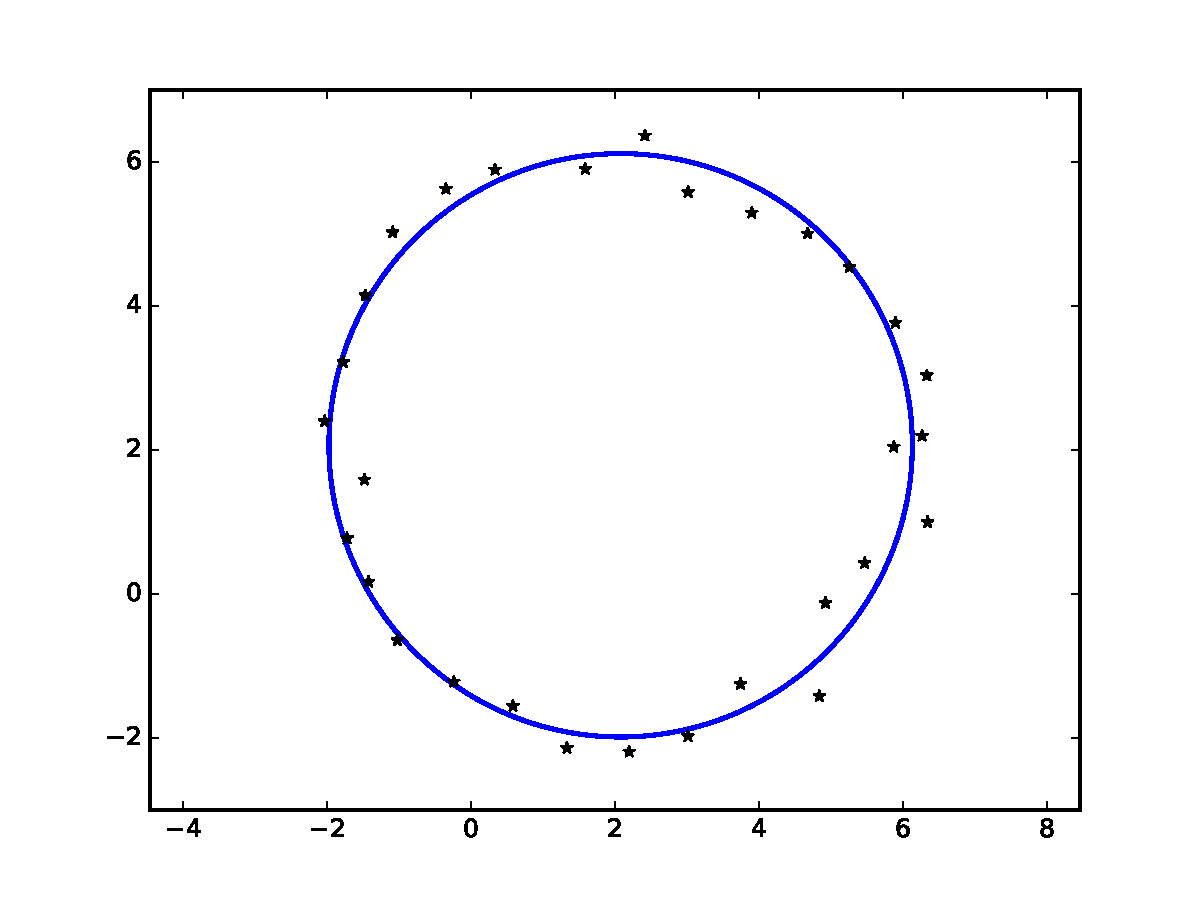
\includegraphics[width=.55\textwidth]{figures/circle_fit_example.pdf}
\end{figure}

\begin{problem}
The general equation for an ellipse is \[ax^2 + bx + cxy + dy + ey^2 = 1.\]
Write a function that calculates the parameters for the ellipse that best fits the data in the file \texttt{ellipse.npy}.
Plot the original data points and the ellipse together, using the following function to plot the ellipse.

\begin{lstlisting}
def plot_ellipse(a, b, c, d, e):
    """Plot an ellipse of the form ax^2 + bx + cxy + dy + ey^2 = 1."""
    theta = np.linspace(0, 2*np.pi, 200)
    cos_t, sin_t = np.cos(theta), np.sin(theta)
    A = a*(cos_t**2) + c*cos_t*sin_t + e*(sin_t**2)
    B = b*cos_t + d*sin_t
    r = (-B + np.sqrt(B**2 + 4*A))/(2*A)

    plt.plot(r*cos_t, r*sin_t, lw=2)
    plt.gca().set_aspect("equal", "datalim")
\end{lstlisting}
\end{problem}

\section*{Computing Eigenvalues} % ============================================

The eigenvalues of an $n \times n$ matrix $A$ are the roots of its characteristic polynomial $\det(A - \lambda I)$.
Thus, finding the eigenvalues of $A$ amounts to computing the roots of a polynomial of degree $n$.
However, for $n \ge 5$, it is provably impossible to find an algebraic closed-form solution to this problem.%
\footnote{This result, called \emph{Abel's impossibility theorem}, was first proven by Niels Heinrik Abel in 1824.}
In addition, numerically computing the roots of a polynomial is a famously ill-conditioned problem, meaning that small changes in the coefficients of the polynomial (brought about by small changes in the entries of $A$) may yield wildly different results.
Instead, eigenvalues must be computed with iterative methods.

\subsection*{The Power Method} % ----------------------------------------------

The \emph{dominant eigenvalue} of the $n \times n$ matrix $A$ is the unique eigenvalue of greatest magnitude, if such an eigenvalue exists.
The \emph{power method} iteratively computes the dominant eigenvalue of $A$ and its corresponding eigenvector.

Begin by choosing a vector $\x_0$ such that $\|\x_0\|=1$, and define the following:
\[\x_{k+1}=\frac{A\x_k}{\|A\x_k\|}\]
If $A$ has a dominant eigenvalue $\lambda$, and if the projection of $\x_0$ onto the subspace spanned by the eigenvectors corresponding to $\lambda$ is nonzero, then the sequence of vectors $\{\x_k\}_{k=0}^\infty$ converges to an eigenvector $\x$ of $A$ corresponding to $\lambda$.

Since $\x$ is an eigenvector of $A$, $A\x = \lambda \x$.
Left multiplying by $\x\trp$ on each side gives $\x\trp A\x = \lambda \x\trp\x$, and hence $\lambda = \frac{\x\trp A\x}{\x\trp\x}$.
This ratio is called the \emph{Rayleigh quotient}.
However, since each $\x_k$ is normalized, $\x\trp\x = \|\x\|^2 = 1$, so $\lambda = \x\trp A\x$.

The entire algorithm is summarized below.

\begin{algorithm}[H] % The Power Method
\begin{algorithmic}[1]
\Procedure{Power Method}{$A$}
    \State $m, n \gets \shape{A}$
        \Comment{$A$ is square so $m = n$.}
    \State $\x_0 \gets \text{random}(n)$
        \Comment{A random vector of length $n$}
    \State $\x_0 \gets \x_0/\|\x_0\|$
        \Comment{Normalize $\x_0$}
    \For{$k = 1,\ 2,\ \ldots,\ N-1$}
        \label{step:power-method-stopping-criterion}
        \State $\x_{k+1} \gets A\x_k$
        \State $\x_{k+1} \gets \x_{k+1}/\|\x_{k+1}\|$
    \EndFor
    \State \pseudoli{return} $\x_N\trp A \x_N,\ \x_N$
\EndProcedure
\end{algorithmic}
\caption{}
\label{Alg:power-method}
\end{algorithm}

The power method is limited by a few assumptions.
First, not all square matrices $A$ have a dominant eigenvalue.
However, the Perron-Frobenius theorem guarantees that if all entries of $A$ are positive, then $A$ has a dominant eigenvalue.
Second, there is no way to choose an $\x_0$ that is guaranteed to have a nonzero projection onto the span of the eigenvectors corresponding to $\lambda$, though a random $\x_0$ will almost surely satisfy this condition.
Even with these assumptions, a rigorous proof of that the power method converges requires tools from spectral calculus.
See Chapter ?? of the Volume I text for details. % TODO: which chapter?

\begin{problem} % Implement the power method.
Write a function that accepts an $n \times n$ matrix $A$, a maximum number of iterations $N$, and a stopping tolerance \li{tol}.
Use Algorithm \ref{Alg:power-method} to compute the dominant eigenvalue of $A$ and a corresponding eigenvector.

Continue the loop in step \ref{step:power-method-stopping-criterion} until either $\|\x_{k+1} - \x_k\|$ is less than the tolerance \li{tol}, or until iterating the maximum number of times $N$.

Test your function on square matrices with all positive entries, verifying that $A\x = \lambda\x$.
Use SciPy's eigenvalue solver, \li{scipy.linalg.eig()}, to compute all of the eigenvalues and corresponding eigenvectors of $A$ and check that $\lambda$ is the dominant eigenvalue of $A$.

\begin{lstlisting}
# Construct a random matrix with positive entries.
>>> A = np.random.random((10,10))

# Compute the eigenvalues and eigenvectors of A via SciPy.
>>> eigs, vecs = la.eig(A)

# Get the dominant eigenvalue and eigenvector of A.
# The eigenvector of the kth eigenvalue is the kth column of 'vecs'.
>>> loc = np.argmax(eigs)
>>> lamb, x = eigs[loc], vecs[:,loc]

# Verify that Ax = lambda x.
>>> np.allclose(A.dot(x), lamb*x)
True
\end{lstlisting}
\end{problem}

% TODO: A note about the convergence of the power method?

\subsection*{The QR Algorithm} % ----------------------------------------------

An obvious shortcoming of the power method is that it only computes the largest eigenvalue and a corresponding eigenvector.
The QR algorithm, on the other hand, attempts to find all eigenvalues of $A$.

Let $A_0 = A$, and for arbitrary $k$ let $Q_kR_k = A_k$ be the QR decomposition of $A_k$.
Since $A$ is square, so are $Q_k$ and $R_k$, so they can be recombined in reverse order.
\[A_{k+1}=R_kQ_k\]
This recursive definition establishes an important relation between the $A_k$.
\[Q_k^{-1}A_kQ_k = Q_k^{-1}(Q_kR_k)Q_k = (Q_k^{-1}Q_k)(R_kQ_k) = A_{k+1}\]
Thus $A_k$ is orthonormally similar to $A_{k+1}$, and similar matrices have the same eigenvalues.
% Furthermore, since each of the $Q_k$ are orthonormal, the computation is numerically stable.
The series of matrices $\{A_k\}_{k=0}^\infty$ converges to the following block matrix.
\[
S =
\left[\begin{array}{cccc}
S_1    & *      & \cdots & *      \\
\0     & S_2    & \ddots & \vdots \\
\vdots & \ddots & \ddots & *      \\
\0     & \cdots &     \0 & S_m
\end{array}\right]
\]

Each $S_i$ is either a $1\times1$ or $2\times2$ matrix.%
\footnote{If all of the $S_i$ are $1\times1$ matrices, then the upper triangular $S$ is called the \emph{Schur form} of $A$.
If some of the $S_i$ are $2\times2$ matrices, then $S$ is called the \emph{real Schur form} of $A$.}
Since $S$ is block upper triangular, its eigenvalues are the eigenvalues of its diagonal $S_i$ blocks.
Then because $A$ is similar to each $A_k$, those eigenvalues of $S$ are the eigenvalues of $A$.

% Second, each iteration of the algorithm transfers some of the ``mass'' from the lower to the upper triangle.
% This is what makes $A_0, A_1, A_2, \ldots$ converge to a matrix $S$ which has the described form.

When $A$ has real entries but complex eigenvalues, $2 \times 2$ $S_i$ blocks appear in $S$.
Finding eigenvalues of a $2 \times 2$ matrix is equivalent to finding the roots of a 2nd degree polynomial, which has a closed form solution via the quadratic equation.
This implies that complex eigenvalues come in conjugate pairs.
%
\begin{align}
% \nonumber S_i=\left[\begin{array}{cc}a&b\\c&d\end{array}\right] \\
\nonumber \det(S_i - \lambda I) =
\left|\begin{array}{cc}
a - \lambda & b           \\
c           & d - \lambda
\end{array}\right|
&= (a - \lambda)(d - \lambda) - bc \\
&= \lambda^2 - ad\lambda + (ad - bc) \label{eq:qr-algorithm-roots}
\end{align}

\subsubsection*{Hessenberg Preconditioning} % - - - - - - - - - - - - - - - - -

The QR algorithm works more accurately and efficiently on matrices that are in upper Hessenberg form, as upper Hessenberg matrices are already close to triangular.
Furthermore, if $H = QR$ is the QR decomposition of upper Hessenberg $H$ then $RQ$ is also upper Hessenberg, so the almost-triangular form is preserved at each iteration.
Putting a matrix in upper Hessenberg form before applying the QR algorithm is called \emph{Hessenberg preconditioning}.

% Second, an iteration of the QR algorithm can be computed in $\mathcal{O}(n^2)$ time on an upper Hessenberg matrix, as opposed to $\mathcal{O}(n^3)$ time on a regular matrix.
% This is because so many entries of an upper Hessenberg matrix are 0.
% If we apply the QR algorithm to an upper Hessenberg matrix $H$, then this speed-up happens in each iteration of the algorithm, since if $H = QR$ is the QR decomposition of $H$ then $RQ$ is also upper Hessenberg.

With preconditioning in mind, the entire QR algorithm is as follows.

\begin{algorithm}[H] % The Power Method
\begin{algorithmic}[1]
\Procedure{QR Algorithm}{$A$}
    \State $m, n \gets \shape{A}$
    \State $S \gets \text{hessenberg}(A)$ \label{step:qr-alg-hessenberg}
        \Comment{Put $A$ in upper Hessenberg form.}
    \For{$k = 0,\ 1,\ \ldots,\ N-1$} \label{step:qr-alg-niters}
        \State $Q, R \gets \text{qr}(S)$ \label{step:qr-alg-qr-S}
            \Comment{Get the QR decomposition of $A_k$.}
        \State $S \gets RQ$
            \Comment{Recombine $R_k$ and $Q_k$ into $A_{k+1}$.}
    \EndFor
    \State \texttt{eigs} $\gets$ \texttt{[]}
        \Comment{Initialize an empty list of eigenvalues.}
    \State $i \gets 0$
    \While{$i < n$}
        \If{$S_i$ is $1 \times 1$} \label{step:qr-alg-S_i-1x1-or-2x2}
            \State Append $S_i$ to \texttt{eigs}
        \ElsIf{$S_i$ is $2 \times 2$}
            \State Calculate the eigenvalues of $S_i$
                \label{step:qr-alg-S_i-eigs}
            \State Append the eigenvalues of $S_i$ to \texttt{eigs}
            \State $i \gets i + 1$
        \EndIf
        \State $i \gets i + 1$
            \Comment{Move to the next $S_i$.}
    \EndWhile
    \State \pseudoli{return} \texttt{eigs}
\EndProcedure
\end{algorithmic}
\caption{}
\label{Alg:qr-algorithm}
\end{algorithm}

\newpage

\begin{problem}
Write a function that accepts an $n \times n$ matrix $A$, a number of iterations $N$, and a tolerance \li{tol}.
Use Algorithm \ref{Alg:qr-algorithm} to implement the QR algorithm with Hessenberg preconditioning, returning the eigenvalues of $A$.

Consider the following implementation details.
\begin{itemize}
    \item Use \li{scipy.linalg.hessenberg()} to reduce $A$ to upper Hessenberg form in step \ref{step:qr-alg-hessenberg}, or use your own Hessenberg function from the previous lab.
    \item The loop in step \ref{step:qr-alg-niters} should run for $N$ total iterations.
    \item Use \li{scipy.linalg.qr()} to compute the QR decomposition of $S$ in step \ref{step:qr-alg-qr-S}, or use your own QR factorization routine from the previous lab (since $S$ is upper Hessenberg, Givens rotations are the most efficient way to produce $Q$ and $R$).
    \item Assume that $S_i$ is $1 \times 1$ in step \ref{step:qr-alg-S_i-1x1-or-2x2} if one of two criteria hold:
    \begin{enumerate}
        \item $S_i$ is the last diagonal entry of $S$.
        \item The absolute value of element below the $i$th main diagonal entry of $S$ (the lower left element of the $2\times 2$ block) is less than \li{tol}.
    \end{enumerate}
    \item If $S_i$ is $2 \times 2$, use the quadratic formula and Equation \ref{eq:qr-algorithm-roots} to compute its eigenvalues.
    Use the function \li{cmath.sqrt()} to correctly compute the square root of a negative number.
\end{itemize}

Test your function on small random symmetric matrices, comparing your results to \li{scipy.linalg.eig()}.
To construct a random symmetric matrix, note that $A + A\trp$ is always symmetric.
% How many iterations are necessary?
% How small does \li{tol} have to be?
% How large can $A$ be?
\end{problem}

\begin{info}
Algorithm \ref{Alg:qr-algorithm} is theoretically sound, but can still be greatly improved.
Most modern computer packages instead use the \emph{implicit QR algorithm}, an improved version of the QR algorithm, to compute eigenvalues.

For large matrices, there are other iterative methods besides the power method and the QR algorithm for efficiently computing eigenvalues.
They include the Arnoldi iteration, the Jacobi method, the Rayleigh quotient method, and others.
We will return to this subject after studying spectral calculus and Krylov subspaces.
\end{info}

\begin{comment} % TODO: WLS, other norms?, QR alg improvements
\newpage

\section*{Additional Material} % ==============================================

\subsection*{Weighted Least Squares} % ----------------------------------------

A \emph{weighted 2-norm} $\|\cdot\|_W$ is defined by the nonsingular matrix $W$ as follows.
\[\|\x\|_W = \|W\x\|_2 = \sqrt{\x\trp W\trp W\x}\]
Typically $W$ is chosen to be a diagonal matrix, in which case the product $W\trp W$ is also diagonal.
Given the overdetermined system $A\x = \b$, the problem of choosing $\widehat\x$ to minimize $\|A\widehat\x - \b\|_W$ is called a \emph{weighted least squares} problem.
This problem has a slightly different normal equation.
\[A\trp W\trp W A \widehat{\x} = A\trp W\trp W \b\]

Letting $C = W A$ and $\z = W \b$, this equation reduces to the usual normal equation.
\[C\trp C \widehat{\x} = C\trp \z\]

Left multiplying $A$ by the diagonal matrix $W$ multiplies the rows of $A$ by the diagonal entries of $W$.
Thus the weighted least squares problem can be solved efficiently by representing $W$ as a 1-D array of its diagonal entries and using array broadcasting.

\begin{lstlisting}
>>> C = np.vstack(w) * A
>>> z = w * b
>>> x = la.lstsq(C, z)[0]
\end{lstlisting}

Weighted least squares is useful when some points in a data set are considered more important than others.
Consider the problem of fitting data to an exponential curve $y = e^{ax} + b$ where points $(x_k,y_k)$ are known.
Taking the natural log of both sides gives $\log(y) = a\log(x) + \log(b)$, so the least squares problem is as follows.
\[
A\x =
\left[\begin{array}{cc}
\log(x_1) & 1 \\
\log(x_2) & 1 \\
\vdots & \vdots \\
\log(x_m) & 1
\end{array}\right]
\left[\begin{array}{c} a \\ \log(b) \end{array}\right]
=
\left[\begin{array}{c}
\log(y_1) \\ \log(y_2) \\ \vdots \\ \log(y_m)
\end{array}\right]
= \b
\]

\subsection*{Using other Norms} % ---------------------------------------------

In these Least Squares problems, we have found best fit lines and ellipses relative to the 2-norm.
It is possible to generalize the idea of best fit curves relative to other norms.
See Figure \ref{fig:lstsq-many-norms} for an illustration of this.

\begin{figure}[h]
    \centering
    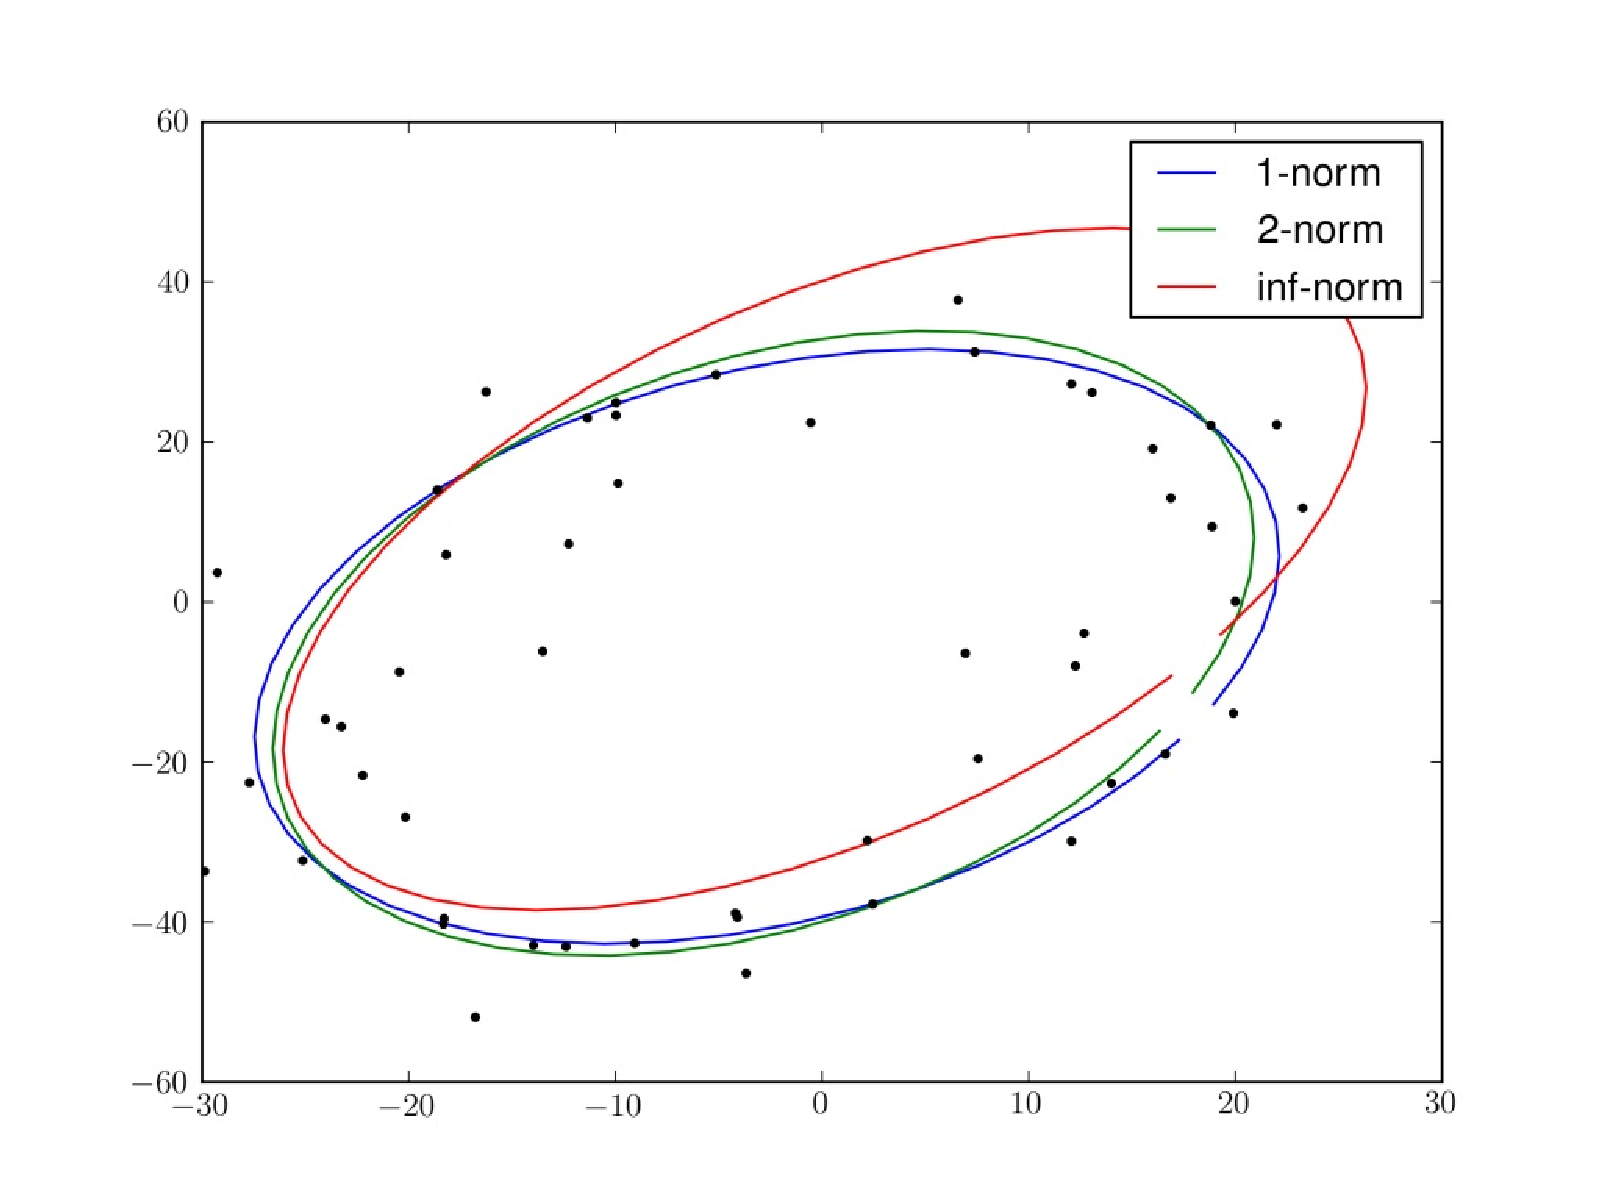
\includegraphics[width=\textwidth]{figures/ellipsefit.pdf}
    % TODO: where did this picture come from? CVXOPT?
    \label{fig:lstsq-many-norms}
\end{figure}

\subsection*{Improvements to the QR Algorithm} % ------------------------------

\end{comment}
